Este capítulo tem como objetivo apresentar uma base teórica mínima de todos os conceitos necessários para o entendimento das demais seções deste trabalho. Primeiramente, serão explicados os conceitos básicos de uma rede neural artificial e suas diferenças em relação a uma rede neural recorrente. Subsequentemente, serão explicados os mecanismos principais de cada modelo utilizado neste trabalho.

\section{Árvores de Regressão}

De acordo com Trevor Hastie et. al. no Livro \textit{The Elements of Statistical Learning}, árvore é uma técnica que pode ser usada para aprendizagem supervisionada. No qual pode ser usado tanto para classificação, árvores de decisão, quanto para regressão, árvores de regressão. Elas são consideradas extremamente poderosas e simples de entender. Basicamente árvores dividem o espaço de características utilizando de regras.

Árvores utilizam de uma algoritmo guloso. Isto é, as melhores escolhas locais fazem parte do melhor resultado global. O algoritmo trata de escolher uma característica e tenta dividir o conjunto de dados em dois utilizando de uma regra na característica e depois de dividir, para conjunto resultante é realizado a mesmo operação. A regra na característica pode ser algo como \texttt{Idade \(\leq\) 40}. O algoritmo para quando não conseguir mais dividir o conjunto de dados.

Existem algumas formas de decidir qual a melhor par, característica e regra, para um conjunto de dados. Escolhido uma característica, é possível determinar a melhor regra que divide o conjunto de dados. Sendo assim, se torna possível comparar os pares resultantes com um custo não exorbitante. A comparação entre os pares pode ser feita de diversas formas, para classificação pode ser usado o \textit{Gini Index} e para regressão pode ser usado Soma do Erros Quadráticos. Uma vez construída a árvore, para utiliza-la basta percorrer a árvore respondendo as regras, assim como mostrado na Figura \ref{figure:tree}.

É importante notar a grande flexibilidade desse modelo de se ajustar ao conjunto de dados. Logo, árvores podem facilmente sobre-ajustar. Isto é, por exemplo, ter em cada folha da árvore um elemento do conjunto de dados. Para resolver isso é possível controlar certos aspectos da construção da árvore. É possível controlar a altura máxima da árvore ou limitar o mínimo de tamanho necessário para se dividir o conjunto. O autor sugere usar o segundo jeito seguido de uma redução da árvore resultante, porém o justo da construção vai depender dos dados.
 
 \begin{figure}[htbp]
    \centering
    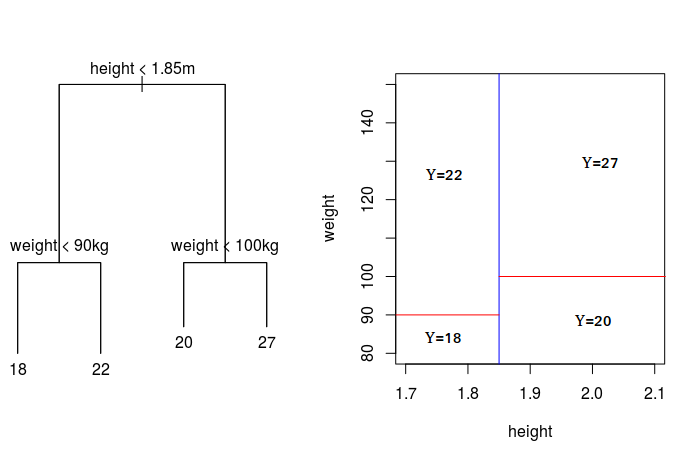
\includegraphics[scale=0.6]{monography/img/models/regression_tree.png}
    \label{figure:tree}
    \caption[Árvore de Regressão Dividindo o Espaço de Resposta]{Árvore de Regressão Dividindo o Espaço de Resposta\footnotemark}
\end{figure}

\footnotetext{\url{https://www.r-bloggers.com/how-random-forests-improve-simple-regression-trees/}}

\section{\acrfull{RF}}

Criado por Leo Breiman em \textit{Random Forest} \cite{Breiman:2001:RF:570181.570182}, \textit{\acrshort{RF}} é um método de aprendizagem de máquina utilizado tanto para classificação quanto para regressão. Segundo o autor, o método é uma combinação de árvores, de decisões ou regressão, onde cada árvore depende de uma amostra aleatória, sendo esta amostra independente do conjunto de dados. Além disso, todas as árvores devem possuir a mesma distribuição. 

A construção das árvores é feita utilizando o método \textit{Bagging} (\textit{\textbf{B}ootstrap \textbf{Agg}regation}), também criado por Leo Breiman em \textit{Bagging Predictors} \cite{Breiman:1996:BP:231986.231989}. Este método gera várias versões de um mesmo modelo e agrega os resultados dos mesmos. As versões do modelo utilizam amostras do conjunto de dados selecionadas aleatoriamente, mas com a mesma distribuição.

Porém, diferente de \textit{Bagging}, \textit{\acrshort{RF}} utiliza mais uma técnica para diminuir o sobre-ajuste (\textit{overfitting}). Há uma modificação no algoritmo de criação das árvores de decisão limitando a quantidade de características (\textit{features}) do conjunto de dados que vai ser utilizada. O autor sugere limitarem a quantidade de características (\textit{q}) para $ \sqrt{q} $, no caso de classificação, ou $ \frac{q}{3} $, no caso de regressão \cite{hastie2005elements}. Além disso, o autor sugere no artigo original que para selecionar a quantidade ideal de características deve se utilizar de estimativas \textit{out-of-bag}, explicadas no artigo.

Como \textit{\acrshort{RF}} é uma combinação de outros modelos de aprendizagem de máquina, ela pode ser classificada como um Comitê de Máquinas (\textit{Ensemble Learning}). A forma como as respostas de cada uma das máquinas são combinadas depende do problema. Para classificação pode ser usado uma votação (voto da maioria) e para um problema de regressão pode ser usado uma média dos valores, assim como mostrado na Figura \ref{figure:random_forest}.

\begin{figure}[htbp]
    \centering
    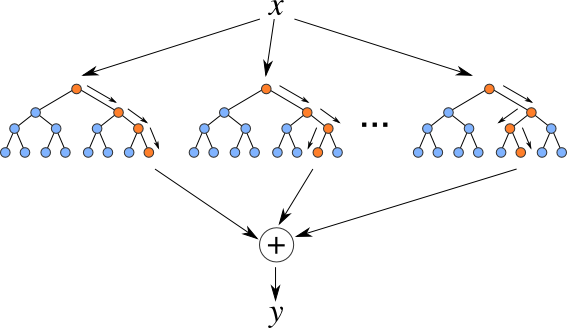
\includegraphics[scale=1.0]{monography/img/models/random_forest.png}
    \label{figure:random_forest}
    \caption[Representação do funcionamento de uma \textit{\acrshort{RF}}]{Representação do funcionamento de uma \textit{\acrshort{RF}}\footnotemark}
\end{figure}

\footnotetext{\url{https://dsc-spidal.github.io/harp/img/4-5-1.png}}

\section{\acrfull{SVM}}
% TODO: adicionar exemplo de uma regressão de 2 dimensões
% TODO: pegar mais referências

\textit{\acrshort{SVM}} foi criado originalmente por Vapnik nos anos 60 e foi evoluindo até se tornar o que é hoje, segundo Smola et. al. \cite{Smola03atutorial}. A ideia básica por trás do método pode ser usada tanto para classificação quanto para regressão. A aprendizagem do modelo é iterativa.

Variável C indica quanto os erros penalizam. Se for baixo, erros não serão muito penalizados e se for alto os erros serão muito penalizados

No caso da regressão, tenta-se criar uma função \(f(x)\) de forma que se \(y(x)\) é a função que perfeitamente descreve o conjunto de dados e \(\epsilon\) seja a dimensão do erro, o ideal seria \(\abs{y(x) - f(x)} \leq \epsilon \).

Além disso, \textit{\acrshort{SVM}} possuem funções \textit{Kernel}, que permitem a mudança de dimensão da entrada para alguma outra de forma rápida. Essa mudança pode aumentar ou diminuir a dimensão da entrada. Assim o modelo não tem que converter o conjunto de dados todo para tentar interpolar em outra dimensão de dados. Existem diversas funções de \textit{Kernel}, como por exemplo, Linear, Não-Linear, \textit{Radial Basis Function} e Polinomial.

Vale notar que algumas funções \textit{Kernel} possuem podem se ajustar quanto ao conjunto de dados. Funções como \textit{Radial Basis Function} e Polinomial possuem uma variável \textit{Gamma} (\(\gamma\)) para controlar esse ajuste. Essa variável determina a influência dos \textit{support vectors} no treinamento. Quanto maior o valor, menor a influência do \textit{support vectors}, quanto menor o valor, maior a influencia. Valores baixos pode levar a uma função que não se ajusta muito ao conjunto de dados, prono a sub-ajuste. Já valores altos podem levar a uma função que se ajusta muito ao conjunto de dados, prono a sobre-ajuste.

\begin{figure}[htbp]
    \centering
    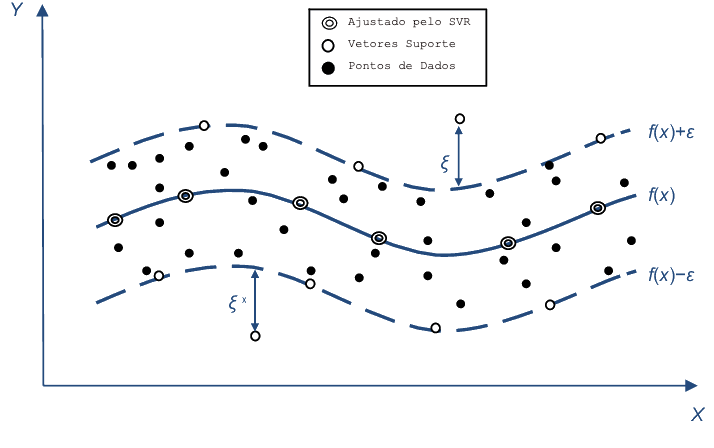
\includegraphics[scale=1.0]{monography/img/models/svr_example.png}
    \label{figure:support_vector_machine}
    \caption[Representação do funcionamento de uma \textit{\acrshort{SVM}}]{Representação do funcionamento de uma \textit{\acrshort{SVM}}\footnotemark}
\end{figure}

\footnotetext{\url{https://www.researchgate.net/figure/Schematic-of-the-one-dimensional-support-vector-regression-SVR-model-Only-the-points_fig5_320916953}}


\section{\acrfull{RNN}}
% RESOURCE: to explain recurrent neural networks (http://d2l.ai/chapter_recurrent-neural-networks/index.html)

% TODO: adiconar referência de onde vc tirou essa explicação

% TODO: Falar que sofre de memória curta e outros defeitos

% TODO: veja esse coisa apra explicar melhor LSTM e RNN (https://www.youtube.com/watch?v=6niqTuYFZLQ)

\textit{\acrshort{RNN}} surgiu da incapacidade de \textit{\acrfull{NN}} de levar em consideração resultados anteriores da rede para computar o resultado atual. Redes neurais artificiais comuns, ou do tipo \textit{feedforward} utilizam apenas do seu estado atual para gerar sua saída. Para exemplificar, tome como exemplo um problema de classificação, onde, a partir de uma imagem de um cachorro, ou gato, uma rede neural deva ser capaz de dizer corretamente qual animal a imagem representa. Para cada rodada de classificação, a imagem utilizada na rodada passada não importa, pois uma não tem relação direta com a outra. 

Porém, existem determinados problemas que exigem certa correlação entre os dados, como por exemplo, interpretar um documento, entender o contexto de um filme, ou avaliar a oscilação de uma bolsa de valores ao longo do tempo. Como descrito por Mitchell em \cite{Mitchell_1997}, \textit{\acrshort{RNN}} são mais adequadas para estas situações, pois nesse tipo de problema, dados isolados não tem tanto significado quanto o conjunto, o que exige um conceito de memória. Para simular este efeito de memória, \textit{\acrshort{RNN}} dispõe de uma arquitetura onde a saída do nó anterior é utilizada como entrada no nó seguinte, juntamente com a entrada nova atual da rede. Para passar estes valores de um nó para o outro, a \texit{\acrshort{RNN}} dispõe de um mecanismo chamado \textit{Hidden Layer} na Figura \ref{figure:rnn} é exemplificada a arquitetura, onde o último resultado utiliza como entrada valores resultantes das últimas execuções.

\begin{figure}[htbp]
    \centering
    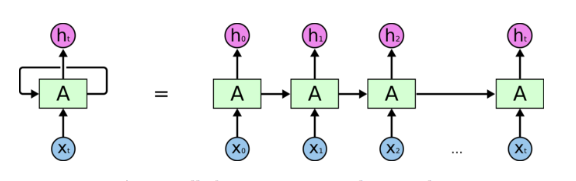
\includegraphics[scale=0.4]{monography/img/models/rnnExample.png}
    \label{figure:rnn}
    \caption[Representação simples do conceito de um RNN]{Representação simples do conceito de uma RNN \footnotemark}
\end{figure}

\subsection{\acrfull{LSTM}}

\acrshort{LSTM} é um método proposto pela primeira vez por Sepp Hochreiter e Jurgen Schmidhuber em \cite{Sepp_1997}. Ele é utilizado para predição de informações que derivam de dados sequenciais e séries temporais, sendo possível encontrar diversos trabalhos na literatura que mostram sua eficiência quando comparado a outros métodos. Como descrito em \cite{Zainab_2018} e em \cite{Xiaolei_2015}, \acrshort{LSTM} é um tipo de \acrshort{RNN} que utiliza de estados anteriores e do estado atual da rede para gerar sua saída. Ao utilizar dos estados anteriores, a \acrshort{RNN} acaba por simular uma memória, melhorando sua capacidade de aprender. 

\begin{figure}[htbp]
    \centering
    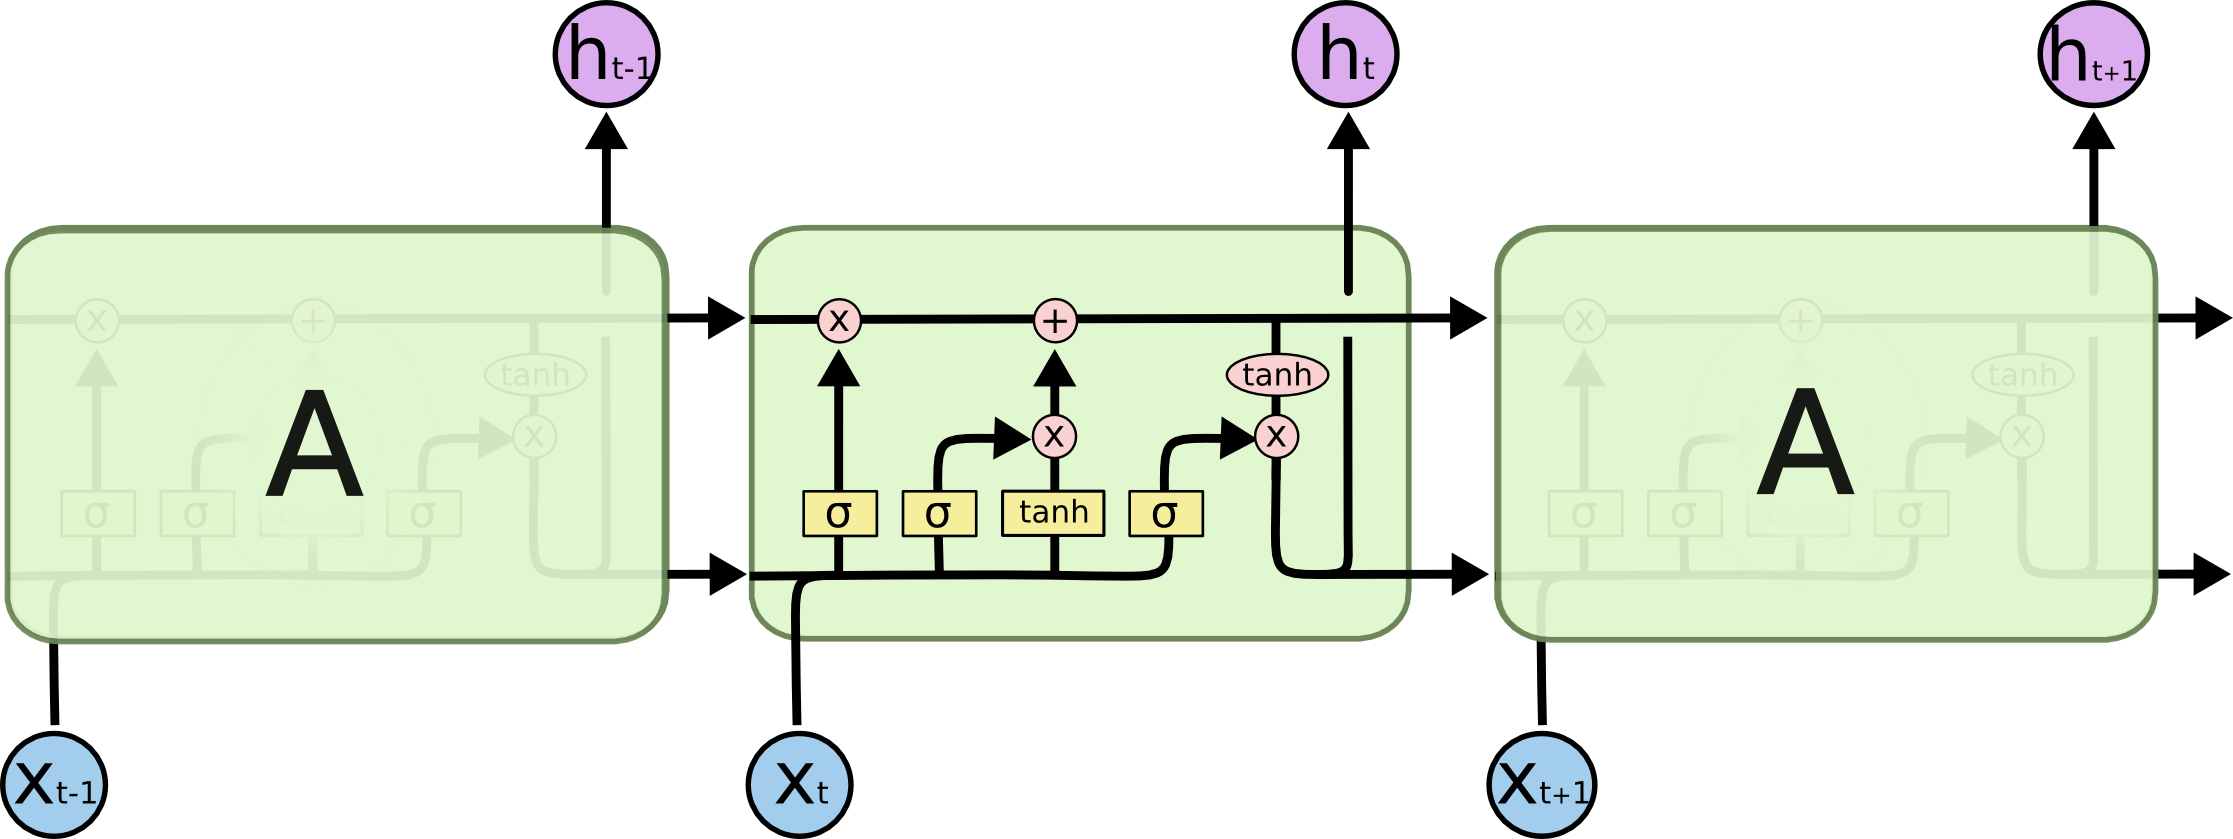
\includegraphics[scale=0.4]{monography/img/models/lstm3.png}
    \label{figure:lstm}
    \caption[Representação de uma arquitetura LSTM]{Representação de uma arquitetura LSTM\footnotemark}
\end{figure}
\footnotetext{\url{https://colah.github.io/posts/2015-08-Understanding-LSTMs/}}


Porém, diferentemente de uma \acrshort{RNN} comum, o LSTM possui uma camada a mais (além da \textit{Hidden Layer}) chamada de \textit{Cell State}. Esta camada é capaz de perceber as características mais latentes dos dados e descartar as menos importantes. Assim, o \acrshort{LSTM} consegue manter as características mais recorrentes na rede por mais tempo que uma \acrshort{RNN} comum. 

Na célula de memória do \textit{\acrshort{LSTM}}, existem estruturas que são responsáveis pela característica de memória a longo prazo e que são responsáveis por controlar a \textit{Cell State}. A Porta de Entrada, a Porta do esquecimento e a Porta de Saída. Abaixo está explicitado como cada um deles funciona:
%TODO: melhorar explicação das portas, principalmente a porta de saída 
%TODO: colocar fórmulas que explicam como o Ct é atualizado
\begin{itemize}
  \item Porta de Esquecimento: A primeira porta de uma célula do \acrfull{LSTM} decide qual informação provinda da célula anterior vai ser descartada. Isso é feito por meio de uma função de ativação sigmoidal que retorna um número entre 0 e 1 para cada valor da célula passada, onde 0 representa total esquecimento daquela informação e 1 total preservação.
  
  \item Porta do Entrada: A segunda porta decide qual informação deve ser atualizada. Para tal decisão são utilizadas duas funções. Primeiro, uma função sigmoid decide quais valores serão atualizados. Depois uma função Tahn cria novos valores candidatos a serem utilizados na atualização.
  \item Porta de Saída: Por fim, a porta de saída efetivamente faz as alterações nos valores da célula de memória atual. Os valores candidatos decididos na Porta de Entrada são colocados no lugar dos valores que devem ser atualizados.
\end{itemize}

% TODO: Falar que podemos responder a quantidade de camadas da LSTM com o problema que RNN tem com back-propagation que o gradiente começa a diminuir exponencialmente. Mas tem que dar uma conferida melhor.

\subsubsection{Funções de ativação}

\subsection{\acrfull{GRU}}


%TODO: explicar diferenca entre porta da reinicializacao e porta da atualizacao, adicionando as fórmulas de cada uma
\textit{\acrshort{GRU}} é um tipo de \textit{\acrshort{RNN}} semelhante ao \textit{\acrshort{LSTM}} e, assim como ele, também faz uso de mecanismos chamados de Portas que possibilitam que a informação seja atualizada ou esquecida ao ser transferida de uma célula para outra. Ou seja, \textit{\acrshort{GRU}} também é capaz de guardar informações importantes na rede de maneira mais eficaz que uma \textit{\acrshort{RNN}} comum. Apesar de parecidos, \textit{\acrshort{LSTM}} e \textit{\acrshort{GRU}} possuem algumas diferenças, como pode ser visto abaixo, o \textit{\acrshort{GRU}} possui apenas a \textit{Hidden Layer} e duas Portas para fazer o tratamento da informação para simular o efeito de memória:

\begin{itemize}
    \item Porta da atualização: A porta de atualização tem um papel semelhante às Portas de Entrada e Porta de Esquecimento do \textit{\acrshort{LSTM}}. Nela, é decidido quais dos valores provindos das células passadas serão adicionados a rede.
    \item Porta da reinicialização: Já o portão de reinicialização decide quanto da informação vinda das células passadas será esquecido.
\end{itemize}

Por ter uma arquitetura mais simples que uma \textit{\acrshort{LSTM}}, o \textit{\acrshort{GRU}} precisa de menos tempo para ser treinado e, geralmente, de menos dados também.

\begin{figure}[htbp]
    \centering
    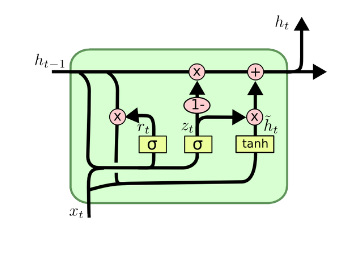
\includegraphics[scale=1.0]{monography/img/models/GRU.png}
    \label{figure:gru}
    \caption[Representação da arquitetura de uma GRU]{Representação da arquitetura de uma GRU\footnotemark}
\end{figure}